

\documentclass{beamer}
\usepackage{graphicx}
\usepackage{listings}
\usepackage{wrapfig}

\usecolortheme{beaver}
\useoutertheme{infolines}
\useinnertheme{circles}
\definecolor{bluish}{RGB}{20,100,200}
\setbeamercolor{frametitle}{fg=bluish}
\setbeamercolor{block title}{fg=bluish}
\setbeamercolor{section in head/foot}{bg=bluish}
\setbeamercolor{author in head/foot}{bg=bluish}
\setbeamercolor{title}{fg=bluish, bg=white}
\setbeamercolor{title in head/foot}{fg=bluish}
\setbeamercolor{date in head/foot}{fg=bluish}


\begin{document}

\newcommand{\tab}{\hspace*{0.4in}} %Paragraph indent
\newcommand{\spc}{\hspace{5pt}} %Word spacing
\newcommand{\vspc}{\vspace*{0.23in}\\} %Interparagraphical jump (skips a line)

\newcommand{\bd}{\textbf} %Bold
\newcommand{\ita}{\textit} %Italic
\newcommand{\ti}{\bf \LARGE} %Heading
\newcommand{\blt}{\begin{itemize}} %Bullet points begin
\newcommand{\finblt}{\end{itemize}} %Bullet Points end.
\newcommand{\eq}{\begin{equation}\label} %numbered equations
\newcommand{\eqf}{\end{equation}}

\newcommand{\pic}[4]{
		\begin{wrapfigure}[#1]{#2}[0px]{#3px}
		\includegraphics[width=#3px,height=300px,keepaspectratio=true]{#4} 			
		\end{wrapfigure}}
		%Form: \pic{height in lines}{Position, left or right entered: l or r}{width in pixels}{Filename}
		
\title{Java Assignment: Peg Board}
\author{Shaun Hegarty}
\institute[DCU]{Dublin City University}

%11(35) - 30-70us 
%51 (675) - 60-100us
%101(2600) - 180-230us
%501 (63000) - 5,400us
%1001 (251000) - ~8,900us
%2001 (1002000) - 18,700us
%5001 (6255000) - 38,100us
%100001 - ~123,000us

%11(35) - 30-70us 
%51 (675) - 60-100us
%101(2600) - 180-230us
%501 (63000) - 5,400us
%1001 (251000) - ~8,900us
%2001 (1002000) - 18,700us
%5001 (6255000) - 38,100us
%100001 - ~123,000us



\section{Intro}

		\frame{\titlepage}


	\begin{frame}
		\frametitle{Problem Definition: The Peg Board}
		\begin{figure}
		\includegraphics[width=10cm]{pegboardlayout}
		\end{figure}
		Consider a board with holes in which coloured pegs can be placed. For this problem we have: 
		\begin{itemize}
			\item pegs of two colours
			\item an equal number of each
			\item a board with enough spaces for all pegs
			\item one additional space which allows for movement
		\end{itemize}
		Movement rules:
		\begin{itemize}
			\item A peg adjacent to the space may move into it
			\item A peg may jump over a peg adjacent to the space into that space
		\end{itemize}	
		
	\end{frame}
		
	\begin{frame}
		\frametitle{Problem Definition: What makes it interesting?}
		For me:
		\begin{itemize}
			\item Pure problem solving exercise
			\item Making a simple game
			\item Some ideas could be extended to 2D and various checkerboard games like draughts
		\end{itemize}
	\end{frame}	
	
\section{Design}
	\begin{frame}
		\frametitle{Design: Breaking it down}
		The aim is to move all pegs of one colour to the other side of the board in the minimum number of steps
		while following the rules.
		
		\begin{figure}
		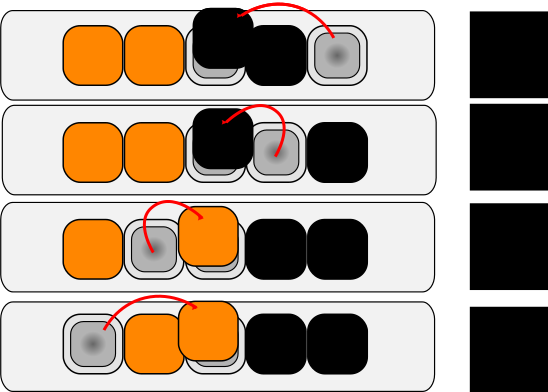
\includegraphics[height=4.5cm]{pegboardmoves}
		\end{figure}
		
		Given the rules we can see that there are only four moves possible at any one time. 
		
		
	\end{frame}
	
	\begin{frame}
		\frametitle{Design: Approaching an Algorithm}
		The problem was solved manually numerous times to determine a pattern.
		\blt
			\item Initial algorithm was effective but inefficient
			\item However, continued efforts revealed a best case algorithm
		\finblt
		\vfill
		A formula for the minimum number of steps:
		\[
		f(n) = 
			\begin{cases} 
				f(n - 2) + n & \textrm{if}\; n \geq 3 \;\textrm{and}\; n \;\textrm{odd}\\
				0 & \textrm{if}\; n < 3
		 	\end{cases}
		\]
		where n is the number of spaces on the board.		
		
	\end{frame}
	
	\begin{frame}
		\frametitle{Design: The Algorithm I - Conditions and Rules}
		\textbf{Starting conditions:} 
		\begin{itemize}
		\item Pegs on either side of the space will be made of one colour only. 
		\item We have a predecided starting direction/colour of which we keep track. 
		\end{itemize}
		\vfill
		\bd{Rules} when determining the next move:
		\begin{itemize}
			\item Each colour can only move in one direction
			\item Prioritize moves of size two, then one. 
			\item If no moves change direction
		\end{itemize}
		
	\end{frame}
	
	\begin{frame}
		\frametitle{Design: The Algorithm II - The Pseudocode}
		The solving loop:
		\begin{itemize}
			\item[] while (not finished)
			\begin{itemize}
				\item[] nextMove()
			\end{itemize}		
		\end{itemize}
		\bigskip
		nextMove() method:
		\begin{itemize}
			\item[] \textbf{if} (current colour can jump over a different colour into hole (in an allowed direction))
			\begin{itemize}
				\item[] move(2 * direction)
			\end{itemize}	
			\item[] \textbf{else if}	(current colour can move into the hole \& be placed adjacent 
			to a different colour (in an allowed direction))
			\begin{itemize}
				\item[] move(1 * direction)
			\end{itemize}
			
			\item[] \textbf{else if}	((hole is at edge of board \& direction is away from the edge of the board) \\
			OR (pieces beyond the space are all in their final positions))
			\begin{itemize}
				\item[] move(1 * direction)
			\end{itemize}
			\item[] \textbf{else} 
			\begin{itemize}
				\item[] change direction
			\end{itemize}

		\end{itemize}
		
		
	\end{frame}
	
	\begin{frame}
		\frametitle{Design: The Algorithm III - A New Pattern Emerges}	
		\begin{columns}[T]
			\begin{column}{.5\textwidth}
				\begin{block}{Another pattern}
				When running the program 
				this symmetric zigzag pattern becomes apparent.
				\\\bigskip
				I framed my logic around the space. Looking at the board as a whole 
				may have led to this approach. 
				\end{block}
			\end{column}
			
			\begin{column}{.5\textwidth}
				\begin{block}{The Zigzag}
				\includegraphics[width=3cm]{pegboardsolved}
				
				\end{block}
			\end{column}
		\end{columns}
	\end{frame}

\section{Analysis}
	\begin{frame}
		\frametitle{Some Analysis}
					

			\begin{figure}
				\includegraphics[height=6cm]{pegboardtime}
			\end{figure}
			The time to complete the solution scaled linearly with the number of moves for large board sizes.	
			
	\end{frame}

\section{Demo}
	\begin{frame}
		\frametitle{Program Demo and that little bit more}
		To complement the solution I created a GUI in which the user can both play the game, or 
		watch the solution presented step by step. \\
		\vfill
		The user can click on any piece, if this piece can make a valid move into the hole, it will. \\
		\vfill
		The user can also increase or decrease the size of the board, and reset the board at any time. 
		
	\end{frame}
\section{Limitations \& Future Work}
	\begin{frame}
		\frametitle{Limitations \& Future Work}
		Limitations
		\blt
			\item The algorithm does not solve the puzzle given an incomplete non-optimal solution. 
		\finblt
		
		Future Work
		\blt
			\item Make implementations of alternate algorithms (the zigzag)
			\item Make the algorithm work for any starting point
			\item The problem can be expanded in numerous ways, such as to a 2D or 3D board which still 
			only has one space for movement
			
		\finblt
	\end{frame}
\section{Reflection}
	\begin{frame}
		\frametitle{Reflection: What did I learn?}

		\blt
			\item Need to step back and look at the bigger picture more often. 
			\item Sometimes miss patterns by breaking things down too quickly.
			\vfill
			\item Graphics2D library in Java. 
			\item In the process I learned about key bindings, mouse listeners,  
			threads and concurrency. 
			\item Made better of use of Github for version control.
		\finblt
		

	\end{frame}
	
	\begin{frame}
		\frametitle{Reflection: What could I have learned?}
		What could I have learned?
		\blt
			\item I only acquired the information I needed to make threads work in my program
			\item I know I didn't touch on vast areas of concurrency such as
			\blt
				\item multithreading
				\item resource locking
				\item synchronisation and more
			\finblt  
			\item I toyed with animating the blocks moving to each new location. I feel it was 
			feasible but (as far as I could tell) I would have had to change my implementation of the 
			pegboard class to make it work effectively. 
		\finblt
	\end{frame}
\section{Conclusion}	
	\begin{frame}
		\frametitle{Conclusion}
		I successfully created an application which could solve the given pegboard problem.\\\medskip
		Additionally I created a GUI which allowed the user to attempt to solve it themselves
		or watch the program solve it. \\\medskip
		I learned a great deal of new content for the latter part as well as some areas in which I can improve myself. 
		
		\bd{Resources Used:}
		\blt 
			\item ZetCode. \ita{Hit testing, moving objects, 2013}[Online]. Available from: 
			http://zetcode.com/gfx/java2d/hitmove/ [Last Accessed 23 April 2015]

			\item Oracle Java Documentation, \ita{How to Use Key Bindings, 2015}[Online]. Available from: 
			http://docs.oracle.com/javase/tutorial/uiswing/misc/keybinding.html [Last Accessed 23 April 2015]
		\finblt
	\end{frame}

\section{Appendix}
	
	\begin{frame}
	\frametitle{Minimum moves}
		Non recursive definition of the minimum moves function:
		\[
			(floor(\frac{n}{2}) + 1)^2 - 1
		\]
		where n is the number of spaces on the board, is odd and $\ge$ 3.
	\end{frame}
	\begin{frame}
	\frametitle{Board Size vs. Moves}
		\begin{figure}
		\includegraphics[width = 10cm]{pegboardbvm}
		\end{figure}
	\end{frame}

\end{document}